\section{Current Research}\label{sec-current}
The effort to enhance source code comprehension has been ongoing since the 
1980s \cite{brooks_towards_1983,letovsky_cognitive_1987} and continues to be an active research field today. In this section we will examine the newer methods of measuring comprehension using comprehension models, inspect current software clarity metrics and the tools in place that use them, review the use of coding style guides in development studios, and study the art of obfuscation and how it can be reversed to help increase code comprehension.

\subsection{Measurement of Comprehension}
Most modern software programs are so complex, relying on multiple modules and libraries, that they become very difficult to understand in their entirety by a programmer. Instead, programmers must rely on a set of cognitive processes that aid in seeking, filtering, and
shaping relevant information for a given programming task \cite{siegmund_measuring_2017}. These comprehension models are described in Section~\ref{sec-models} as: top-down, bottom-up, and integrated.

Siegmund et al \cite{siegmund_understanding_2014}, uses a functional magnetic resonance imaging (fMRI)
scanner to show that bottom-up chunking techniques increase subjects overall code comprehension. The
researchers were able to replicate their original results, and further solidify their original findings of
the effectiveness of chunking techniques in bottom-up comprehension models \cite{siegmund_measuring_2017,
siegmund_understanding_2014}. As shown in Figure \ref{fig:fMRI}, their experiments found that the 
cognitive centers of the brain activated more intensely when using chunking methods of bottom-up
comprehension, than when using top-down comprehension models. Their results showed that the areas of the
brain linked to cognition and understanding (Brodmann areas), are more active during chunking practices
than they are during top-down comprehension. 

Yeh et al \cite{yeh_detecting_2017}, also found that when using an electroenchephalogram (EEG) subjects
had smaller alpha and theta band magnitudes during comprehension of non-confusing code snippets versus
confusing code snippets. The non-confusing micro-patterns were presented in a method that was similar to
bottom-up models, where the snippet was small enough that the participants of the experiment were able to
determine the smaller pieces (chunks) first and apply that knowledge to the idea that made up the overall
purpose of the program. Their experiment was setup to measure the difference in theta and alpha band
magnitudes over the 8 channels that are related to cognitive load, as indicated by the red circle shown in
Figure \ref{fig:EEG}. The results showed that smaller non-confusing code patterns were easier for subjects
to understand and these findings fit well with the bottom-up approach of comprehension models.

While the current research in Software comprehension seems to lead towards a bottom-up model of
comprehension being the most effective \cite{siegmund_measuring_2017, siegmund_understanding_2014, yeh_detecting_2017, nakagawa_quantifying_2014}, it should be noted that source code is a language and can
be read as such. Angosto et al \cite{angosto_pdf_nodate} studied general reading comprehension when the
subject does not have prior knowledge of the material. In their experiments it was shown that without
prior knowledge that a broad overview (top-down model approach) of the material was best suited to the
subject's cognitive understanding. 

These experimental results show that a version of the bottom-up comprehension model seems to work best when reading source with a bit of prior knowledge of the code, and if there is no prior knowledge of the source a top-down model works well. Combining the findings of this research would suggest that an integrated model of comprehension would be a future area of research in code comprehension. As research continues in this area, there will be a more solid confirmation of what types of comprehensional model will be the most useful in designing automatic tools and metrics to make the job of software readability easier.

\begin{figure}[ht]
\centering
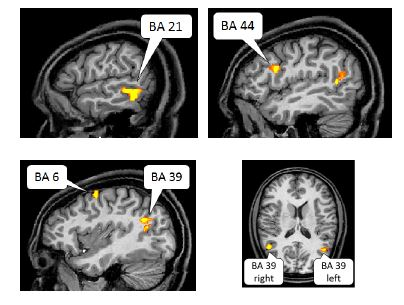
\includegraphics[scale=0.75]{images/fMRI}
\caption{Functional MRI scans that show activation in the Brodmann-areas during bottom-up comprehension.}
\label{fig:fMRI}
\end{figure}

\begin{figure}[ht]
\centering
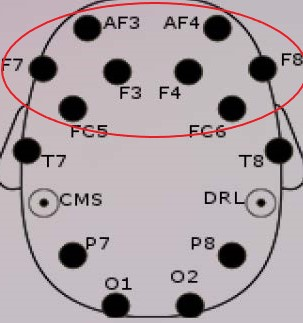
\includegraphics[scale=0.75]{images/EEG}
\caption{Electrode positioning of EEG headset in Yeh et al experiment with the 8 cognitive load channels highlighted.\cite{yeh_detecting_2017}}
\label{fig:EEG}
\end{figure}



\subsection{Software Clarity Metrics}
To improve program comprehension, there has also been research done in software readability and clarity
metrics. Metrics are a measurement by which an attribute's state is determined. Using these determinations
we can gauge the effectiveness of software readability and comprehension applications, with the hopes of
improving the behavior that is desired. Maurya states that the factors that influence understandability
characteristics in comprehending software are an internal software quality and an internal process of
human influences\cite{maurya_software_nodate}. As shown in Figure \ref{fig:models}, the programmers
knowledge base and mental representation of the program under analysis help to aid the assimilation
process during comprehension.  
  
Comprehension of source code can often be equated to the effective readability of the source, meaning that
the easier it is for developers to read the code tends to directly effect how easily the developers
understand it \cite{dorn_general_nodate}. Work on software clarity metrics has shown that factors such as
the number of identifiers, the number of
statements, and the amount of branching have an impact on code comprehension~\cite{brooks_towards_1983}.

In more current research the length of identifiers was not shown to have an impact on comprehension, while
the amount of characters per line was shown to have a significant impact \cite{buse_metric_2008}. By improving the metrics that are used to determine the effectiveness of comprehension in specific attributes
commonly used in source code, we are able to write more efficient automated methods for determining a
programs overall readability.  
\subsection{Coding Style Guides}
A rather simple method of ensuring better program comprehension in a project is to follow a programming
language style guide. Each coding style is different because it is how a programmer's code is assembled to
look and is often influenced by the developer’s particular experiences (IDEs used, etc.) and can even vary
from language to language. Coding style guides provide an overarching standard methodology for the layout
and the usage for various pieces of language functionality in a project. An example from the Google C++ style guide is shown in Figure \ref{fig:style}.

\begin{figure}[ht]

\begin{tcolorbox}

\scriptsize 
\begin{Verbatim}
     \textbf{\textcolor{OliveGreen}{(a) Bad initialization:}}                             
1. int i;          
2. i = f();
3. //bad - initialization separate
   //      from declaration
     \textbf{\textcolor{OliveGreen}{(b) Good initialization:}}
1. int j = g();
2. //Good - initialization includes declaration
\end{Verbatim}
\end{tcolorbox}

\caption{Excerpt from Google C++ coding style guide regarding the declaration and initialization of local variables \cite{google_google_2011}.}
\label{fig:style}
\end{figure}


\begin{figure*}[!ht]
\begin{tcolorbox}

\scriptsize 
\begin{Verbatim}
   
   private void CalculatePayroll(SpecialList, employeeGroup) \{
     while(employeeGroup.HasMore())\{
         employee = employeeGroup.GetNext(true);
         employee.UpdateSalary();
         DistributeCheck(employee);
     \}
   \}    
\end{Verbatim}
\end{tcolorbox}
\caption{An example of source code containing vulnerability.
\label{fig-blind}}
\end{figure*}

Style guides help to ensure that all programmers adhere to the same coding standard, by keeping all the pieces 
of the project consistent. This consistency allows for a quicker understanding of the source code by
all members of the project. Using standards and heavily documenting the program helps to ensure future developers are well equipped to understand the source.

Coding style guides are popular in industry and large scale open-source projects 
\cite{google_google_2011,weinberger_google_2011,doland_c_1994,torvalds_linux_nodate, van_rossum_pythonstyle-pep_2001} because they provide a map that 
allows anyone to quickly get into the meaning of the code by providing detailed directions to follow. They are more 
than just a document, and have helped to change the way that software projects are developed by providing
a uniform practice which allows any developer to just jump right in on the project
\cite{gale_collaborative_1996}.

A good code style guide is like following a turn-by-turn GPS to a destination since
there is no need to take the road less traveled, instead it is guaranteed that instead the most direct route to the final goal is taken. Style guides help new 
developers to the team catch up quickly \cite{google_google_2011}, provide significantly less overhead maintenance \cite{torvalds_linux_nodate}, and help to keep all 
modules looking cohesive \cite{doland_c_1994}. With the knowledge of what practices work best, newer style guides may be created to maximize the potential for source code comprehension.


\subsection{Obfuscation}
After researching all efforts that have gone into making code easier to understand it is worth noting that not all developers wish to make their code easier to read. In fact, many strive to make their code as
difficult as possible to prevent reverse engineering and theft of their coding ideas. In the fast
paced world of software development, many companies rely on confusion in their code in order to increase security from hacking and code theft. 

Source code obfuscation is essentially a protection mechanism, for vulnerable code as shown in Figure \ref{fig-blind}, that is widely used to limit the possibility of malicious reverse
engineering or attack activities on a software system \cite{ceccato_effectiveness_2009}.
Obfuscation is a method that is inversely related to code comprehension, so much that the ideals of
obfuscation in themselves can help us to understand what makes code confusing in the first place.  
Obfuscated code is by design confusing code, and the methods that are used to ensure it is confusing
can lead to a better understanding of unintentionally confusing code.

As shown in Figure \ref{fig:Transforms}, obfuscation transformations can be classified into three groups: \textbf{layout obfuscations} which remove
relevant information from the code without changing its behavior; \textbf{data obfuscations} which transform application
data and data structures (e.g., data encoding, data splitting); and, \textbf{control-flow obfuscations} which alter the original flow of the application \cite{collberg_taxonomy_1997}.

The technique of obfuscation that is of particular interest is identifier renaming, which is an instance of layout obfuscation.
It removes relevant information from the code by changing the names of classes, fields and operations into
meaningless identifiers \cite{ceccato_effectiveness_2009}, as shown in Figure \ref{fig:test}. By reversing this process, it is apparent that identifier naming conventions can increase software clarity and overall code comprehension.

\begin{figure*}[ht]
\centering
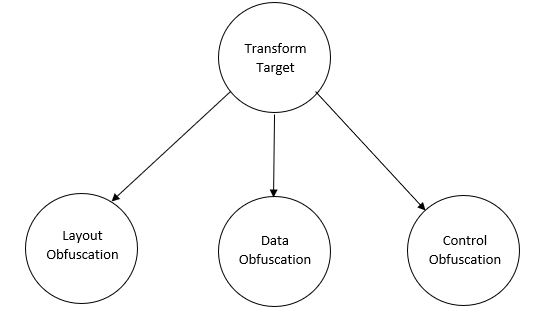
\includegraphics[scale=.7]{images/Obfuscate}
\caption{Classifications of Obfuscation Transforms}
\label{fig:Transforms}
\end{figure*}

\begin{figure*}
\begin{tcolorbox}
\centering
\begin{subfigure}{.5\textwidth}
  \centering
  %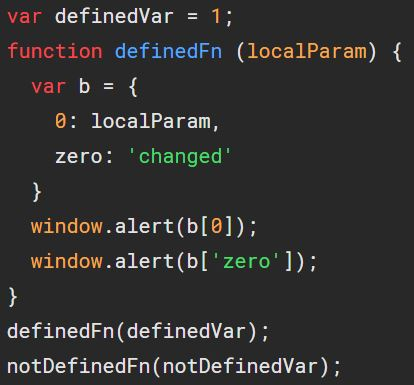
\includegraphics[width=.6\linewidth]{images/ID1}
  \begin{Verbatim}
  var definedVar = 1;
  function definedFn(localParam) \{
    var b = \{
      0: localParam,
      zero: 'changed'
    \}
    window.alert(b[0]);
    window.alert(b['zero']);
  \}
  definedFn(definedVar);
  notDefinedFn(notDefinedVar);
  \end{Verbatim}
  \caption{Normal Identifiers}
  \label{fig:sub1}
\end{subfigure}%
\begin{subfigure}{.5\textwidth}
  \centering
  %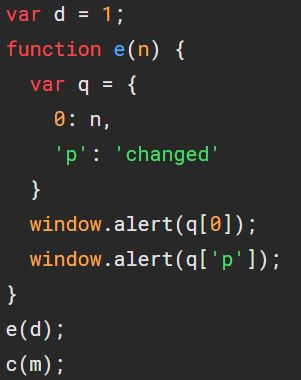
\includegraphics[width=.5\linewidth]{images/ID2}
  \begin{Verbatim}
  var d = 1;
  function e(n) \{
    var q = \{
      0: n,
      'p': 'changed'
    \}
    window.alert(q[0]);
    window.alert(q['p']);
  \}
  e(d);
  c(m);
  \end{Verbatim}
  \caption{Obfuscated Identifiers}
  \label{fig:sub2}
\end{subfigure}
\end{tcolorbox}
\caption{An example of Identifier Obfuscation}
\label{fig:test}
\end{figure*}
There is so much interest in the obfuscation of code that there are a number of contests in which the
sole purpose is to make the source code as confusing as possible. These contests span a majority of
languages and show that obfuscation is something that is not only possible, but desired in many facets
of the software development industry. The oldest contest that is still running is the International
Obfuscated C Code Contest (IOCCC)\footnote{\url{https://www.ioccc.org/}}, which has been around since 1984. The winners of the IOCCC strive to
create code that is functional but incredibly hard to follow, as seen in Figure \ref{fig:IOCCC}. Winners of
the contest often use little known tricks, such as using the C preprocessor to do unintended things, or
they tend to avoid using common constructs that are available in C in favor of more obscure methods 
that achieve the same results.  


\begin{figure}[!ht]
\scriptsize
\centering
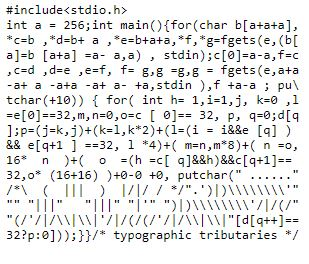
\includegraphics[scale=1.0]{images/IOCCC}
\begin{comment}
\begin{Verbatim}[frame=none]
#include<stdio.h>
int a = 256;int main()\{for(char b[a+a+a],
*c=b ,*d=b+ a ,*e=b+a+a,*f,*g=fgets(e,(b[
a]=b [a+a] =a- a,a) , stdin);c[0]=a-a,f=c
,c=d ,d=e ,e=f, f= g,g =0,g = fgets(e,a+a
-a+ a -a+a -a+ a- +a,stdin ),f +a-a ; pu\\
tchar(+10)) \{ for( int h= 1,i=1,j, k=0 ,l
=e[0]==32,m,n=0,o=c [ 0]== 32, p, q=0;d[q
];j=k,k=l,m=n,n=o,p=(j)+(k* 2 )+(l =(i = 
e[ q]&&i ) &&e[q +1 ]== 32,l*4)+(m* 8 )+(
16*  n  )+(  o  =(h =c[ q]&&h)&&c[q+1]== 
32,o* (16+16) )+0-0 +0, putchar(" ......"
/*\  (  |||  )  |/|/ / */".')|)\\\\\\\\'"
"" "|||"   "|||" "|'" ")|)\\\\\\\\'/|/(/"
"(/'/|/\\|\\|'/|/(/(/'/|/\\|\\|"[d[q++]==
32?p:0]));\}\}/* typographic tributaries */
\end{Verbatim}
\end{comment}
\caption{A winner of the 2018 IOCCC \cite{noauthor_international_nodate}.}
\begin{comment}
\yanyan{ 
Also please check some of the backslashes. 
They need to have an escape char.}\end{comment}

\label{fig:IOCCC}
\end{figure}

In quantifying program obfuscation, we can also quantitatively approach code defactoring which leads us
towards increased code comprehension\cite{anckaert_program_2007, capiluppi_code_2012}. By reversing the
principles of obfuscating code we see that there are certain aspects that help to make
code really confusing and may be able to update style guids to help remove those practices in production
code when we wish to increase code comprehension. 